\chapter{Event selection}
\label{chap:eventselection}
The event selection has been optimized for the EW VV+jj signals against the background processes.
First the object definition is shown in section~\ref{sec:object}, then the detail of the whole event selection is presented in section~\ref{sec:eventselection}.
\section{Object definition}
\label{sec:object}
In this section object definition employed in the analysis is shown.
\subsection{Triggers}
Trigger selection is firstly applied in order to select events in interest.
The triggers applied depend on the channel and on the data taking period. 
The trigger selection is done using single-electron or single-muon triggers.
The list of the trigger names applied in this analysis is summarized in table~\ref{tab:Triggers}.
\begin{table}[H]
\begin{center}
\resizebox{1.0\textwidth}{!}{
\begin{tabular}{|l|c|c|c|}
\hline
\multirow{2}{*}{Data-taking period} & \multirow{2}{*}{$e\nu qq$ and $eeqq$ channels} & $\mu\nu qq$ ($\pt(\mu\nu)<150\,\GeV$) & $\mu\nu qq$ ($\pt(\mu\nu) > 150\,\GeV$)  \\
&& and $\mu\mu qq$ channels& and $\nu\nu qq$ channels\\
\hline
\hline
\multirow{3}{*}{\centering {2015}} & HLT\_e24\_lhmedium\_L1EM20 OR & HLT\_mu20\_iloose\_L1MU15 OR & \multirow{3}{*}{ HLT\_xe70 } \\
 & HLT\_e60\_lhmedium OR & HLT\_mu50 & \\
 & HLT\_e120\_lhloose & & \\
\hline
\multirow{2}{*}{\centering {2016a (run $< 302919$)}} & HLT\_e26\_lhtight\_nod0\_ivarloose OR & HLT\_mu26\_ivarmedium OR  & \multirow{3}{*}{ HLT\_xe90\_mht\_L1XE50 } \\
 & HLT\_e60\_lhmedium\_nod0 OR & HLT\_mu50 &  \\
\multirow{2}{*}{($L<1.0\times10^{34}\,{\textrm cm}^{-2}\,{\textrm s}^{-1}$)} & HLT\_e140\_lhloose\_nod0 & & \\
 & HLT\_e300\_etcut & & \\
\hline
{\centering {2016b (run $\geq 302919$)}} & \multirow{2}{*}{same as above} & \multirow{2}{*}{same as above}  &  \multirow{2}{*}{HLT\_xe110\_mht\_L1XE50} \\
($L<1.7\times10^{34}\,{\textrm cm}^{-2}\,{\textrm s}^{-1}$) & & &\\
\hline
{\centering {2017}} & same as above & same as above  &  HLT\_xe110\_pufit\_L1XE55 \\
\hline
{\centering {2018}} & same as above & same as above  &  HLT\_xe110\_pufit\_xe70\_L1XE50  \\
\hline
\end{tabular}
}
\caption{The list of triggers used in the analysis.} 
\label{tab:Triggers}
\end{center}
\end{table}

\subsection{Leptons}
Electrons are required to have: $p_\mathrm{T}$ > 30~GeV in 1-lepton channel and $p_\mathrm{T}$ > 7~GeV in the 2-lepton channel, and pseudorapidity $|\eta|$ < 2.47 while muons should satisfy: $p_\mathrm{T}$ > 30~GeV in the 1-lepton channel and $p_\mathrm{T}$ > 7~GeV in 2-lepton channel, and $|\eta|$ < 2.5. 
``Tight" identified electron and muon described in chapter~\ref{chap:reconstruction}, is used for the 1-lepton channel, while ``Loose" electron and muon candidate is used for the 2-lepton channel.
Electrons and muons are required to have a transverse impact parameter significance relative to the beamline ($|d_0|/\sigma_{d_0}|$) smaller than 5 and 3, respectively, and a longitudinal impact parameter $|z_0 \times sin \theta | < 0.5$~mm relative to the primary vertex.
\subsection{Jets}
\noindent\textbf{\sf{Small-R jets}} \\ 
Small-R jets are reconstructed using the anti-$k_\mathrm{T}$ algorithm from the PFllow objects, described in chapter~\ref{chap:reconstruction}.
Small-R jets in $|\eta|$ < 2.5 (central jets) are required to have a $p_\mathrm{T}$ > 20~GeV while jets with $|\eta|$ > 2.5 (forward jets) requires $p_\mathrm{T}$ > 30~GeV. 
In order to reassure that the selected jets are coming from the hard-scatter vertex, the ``tight" working point JVT cut, introduced in chapter~\ref{chap:reconstruction}, is applied for jets with $p_\mathrm{T}$ < 60~GeV and $|\eta|$ < 2.4. The ``loose" working point fJVT cut is also applied to the jets outside the tracking coverage (2.5 < $|\eta|$ < 4.5).  \\ 
\\
\noindent\textbf{\sf{Large-R jets}} \\ 
Large-R jets are required to have $p_\mathrm{T}$ > 200~GeV, $|\eta|$ < 2.0 and $m > $50~GeV. 
In order to identify a large-R jet coming from a W/Z boson decay, a 3-variable W/Z tagger described in chapter~\ref{chap:reconstruction} is employed. 
\section{Event selection}
\label{sec:eventselection}
%overview
Common preselection cuts are applied including event cleaning and the trigger requirements, followed by a specific event selection to each of the 0,1,2-lepton channels.
For the main event selection, first the $W/Z$ boson decaying leptonically is selected, then pair of forward jets to enhance the VBS topology is selected, and finally the signal region (SR) and the control region (CR) are defined by the hadronically decaying W/Z boson reconstruction. Several CRs dedicated to main background processes (V+jets, $t\bar{t}$) are defined separately, and they are used to estimate the normalization of the simulated background events from the data.

%\section{Preselection}
%Firstly some pre-selection on the Triggers, event cleaning selections are applied to get the available events and to reject the problematic events. The same selection is applied both for data and MC samples.
%The selections with respect to the number of jets and leptons at minimum is applied, as summarized in Table~\ref{tab:presel_CxAOD}.
%\begin{table}[H]
%\begin{center}
%\resizebox{0.55\textwidth}{!}{
%\begin{tabular}{|l|c|}
%\hline\hline
%\multicolumn{2}{|c|}{ Common } \\
%\hline\hline
%Trigger & listed in Table~\ref{tab:triggers} \\
%\hline
%Event Cleaning & listed in Section~\ref{subsec:event_cleaning} \\
%\hline
%Number of jets & $N_j \geq 2$ or $N_J^{\textrm{LCTopo}} \geq 1$ \\
%\hline\hline\hline
%%\multicolumn{2}{|c|}{ 1-lepton channel } \\
%%\hline
%%Number of Tight leptons   & $=1$ \\
%%\hline
%%Number of additional Loose leptons   & $=0$ \\
%%\hline
%%\ptlv                     & $>75\,\GeV$ \\
%%\hline\hline
%\multicolumn{2}{|c|}{ 2-lepton channel } \\
%\hline\hline
%Number of Loose leptons   & $=2$ \\
%\hline
%The leading lepton \pt    & $> 25$~GeV \\
%\hline\hline
%%\multicolumn{2}{|c|}{ 0-lepton channel } \\
%%\hline\hline
%%Number of Loose leptons   & $= 0$ \\
%%\hline
%%\met                      & $> 140\,\GeV$ \\
%%\hline\hline
%\end{tabular}
%}
%\end{center}
%\caption{List of the pre-selections applied.
%%Definitions of Tight and Loose leptons are found in Sections~\ref{subsec:electron_selection}--\ref{subsec:muon_selection}.
%%$N_j$ is the number of signal- and VBF-jets defined in Section~\ref{subsec:jet_selection}.
%%$N_J^{\textrm{LCTopo}}$ is the number of large-R jets with $\pt>200\,\GeV$ and $\left| \eta \right| < 2.5$.
%} \label{tab:presel_CxAOD}
%\end{table}

\subsection{Selection of the leptonically decaying boson}
The selection to reconstruct the leptonically decaying $W/Z$ boson is applied separately in each lepton channel. \\ \\
\noindent\textbf{\sf{0-lepton}}  \\
In the 0-lepton channel, a high missing transvers momentum $E^{miss}_\mathrm{T}$ is expected to originate from two neutrinos in the final state. 
Cuts on $E^{miss}_\mathrm{T}$ ( $>$ 200~GeV) and $E^{\mathrm{miss,track}}_\mathrm{T}$ ( $>$ 50~GeV) is applied. 
The QCD-induced multijet background with fake $E^{miss}_\mathrm{T}$ due to the mis-reconstruction and momentum resolution of the jets is significant in the 0-lepton channel. 
To suppress its contribution, several cuts are applied related to the direction of $E^{miss}_\mathrm{T}$ and the jet: $\Delta\phi(\met,\mpt) < \pi/2$, $\min(\Delta\phi(\met,j)) > \pi/6$ and, $\Delta\phi(\met, V_{had}) > \pi/9$. The fake $E^{miss}_\mathrm{T}$ contribution can be ignored after this selction. \\ \\ 
\noindent\textbf{\sf{1-lepton}}  \\
One tight-lepton with $p_\mathrm{T} > 28~\mathrm{GeV}$ and $E^{miss}_\mathrm{T} > 80~\mathrm{GeV}$ is required. In 1-lepton channel there are significant contribution from t$\bar{\mathrm{t}}$ background hence b-veto is applied to all small-R jets to reduce its contribution.\\ \\
\noindent\textbf{\sf{2-lepton}}  \\
Two same flavor loose-leptons satisfying $p_\mathrm{T}$ > 27~GeV ( $p_\mathrm{T}$ > 27~GeV) for the leading (sub leading) one 
and an invariant mass of the lepton system ( m$_{ll}$ ) close to the Z boson mass are requested. Figure~\ref{fig:2lepLeptons} shows a peak of the invariant mass reconstructed by two selected leptons around the Z boson mass. Depending on the lepton pair (ee, $\mu\mu$) different mass
window requirements are applied; for electrons, $83<m_{ee}<99 ~\mathrm{GeV}$ is applied, for muons $p_{\mathrm{T},ll}$-dependent mass window is required in order to recover the dimuon mass resolution degradation at high-$p_{T,ll}$ \cite{EXOT-2016-29}:
\begin{equation*}
\left(85.6-0.0117 p_{\mathrm{T}, \ell \ell}\right)<m_{\mu \mu}<\left(94.0+0.0185 p_{\mathrm{T}, \ell \ell}\right) ~\mathrm{GeV}
\end{equation*}
In addition, muons are required to have opposite charges. 
The opposite charge requirement is not requested for electrons which are more susceptible to charge mis-identification due to the conversions of photons from bremsstrahlung. After this selection most of the background process exist is Z+jets.
%Data and MC distributions of relevant lepton distribution at the early stage of the selection are shown in Figure~\ref{fig:2lepLeptons}.
\begin{figure}[H]
    \centering
    %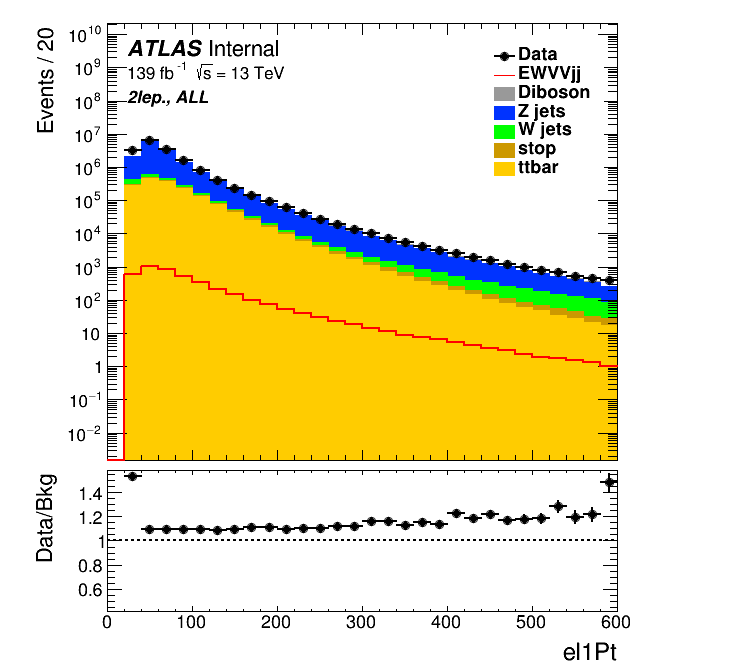
\includegraphics[width=0.4\textwidth]{figures/2lep/dataMC/C_0ptag1pfat0pjet_0ptv_ALL_el1Pt_Log}
    %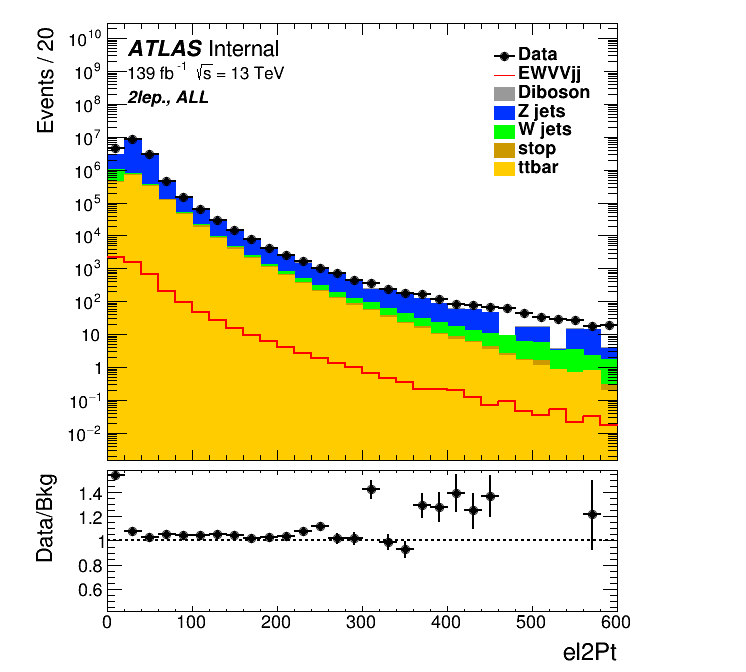
\includegraphics[width=0.4\textwidth]{figures/2lep/dataMC/C_0ptag1pfat0pjet_0ptv_ALL_el2Pt_Log} 
    %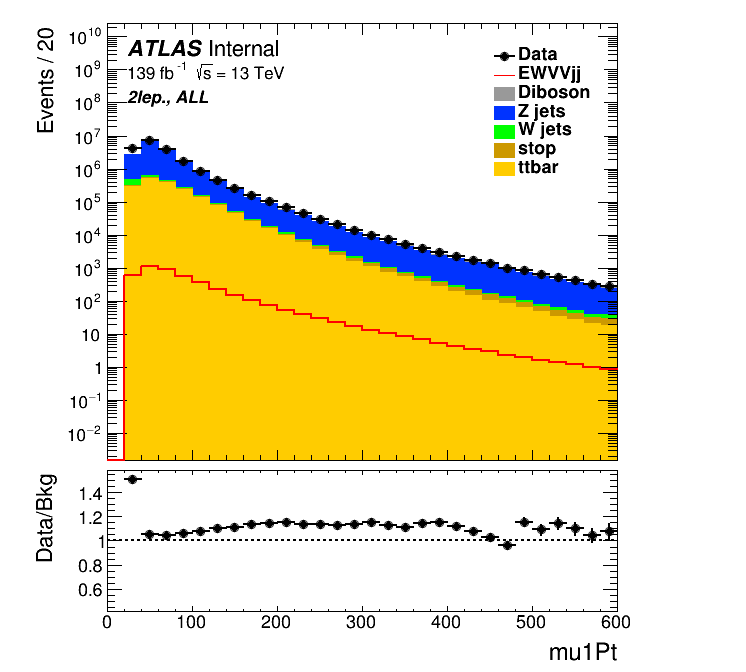
\includegraphics[width=0.4\textwidth]{figures/2lep/dataMC/C_0ptag1pfat0pjet_0ptv_ALL_mu1Pt_Log}
    %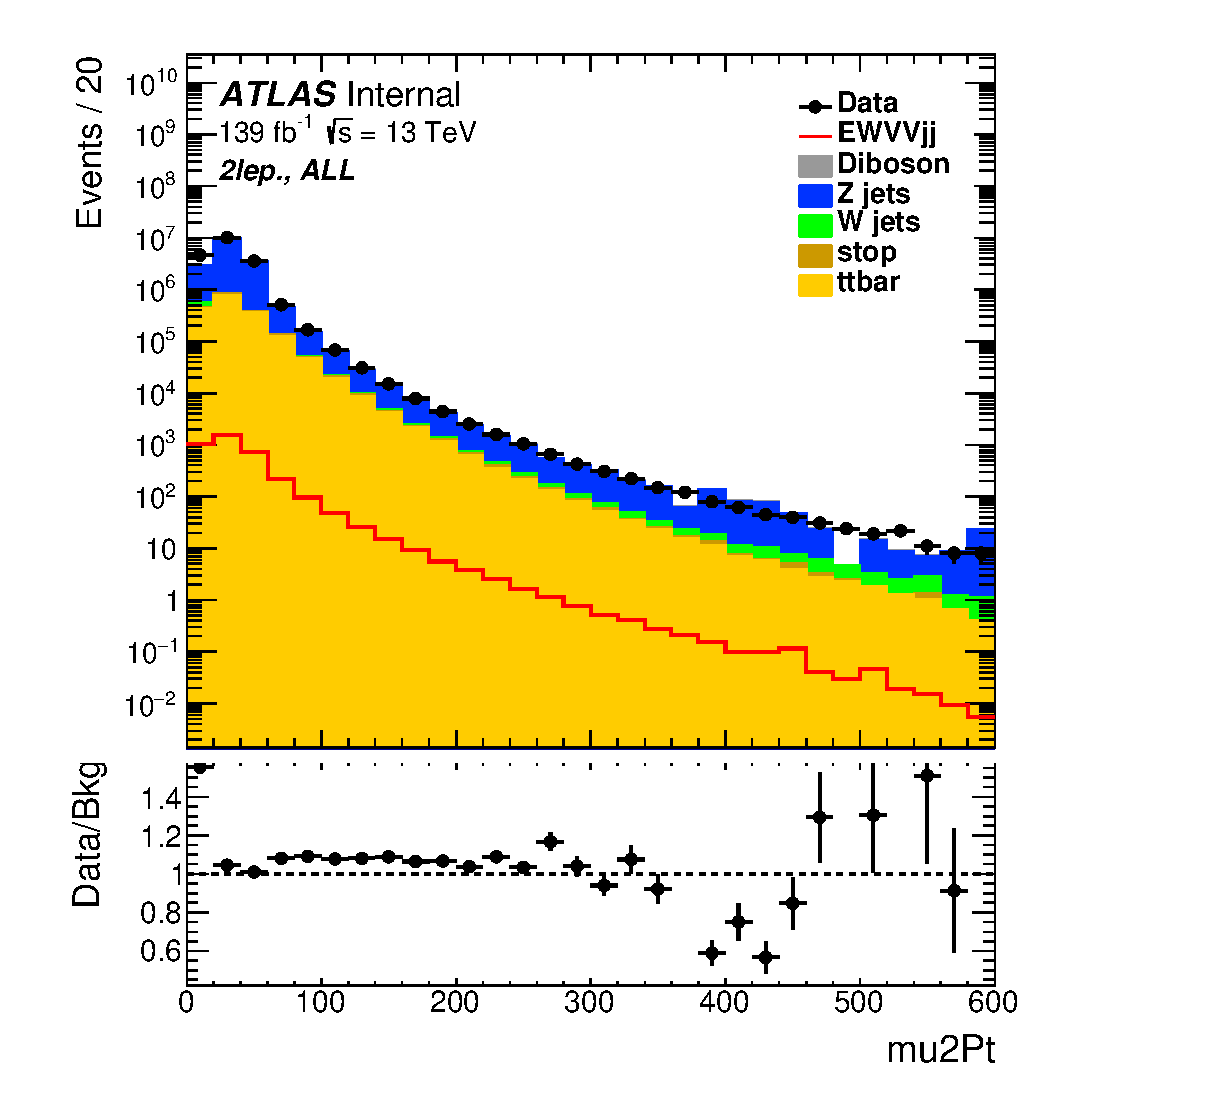
\includegraphics[width=0.4\textwidth]{figures/2lep/dataMC/C_0ptag1pfat0pjet_0ptv_ALL_mu2Pt_Log} 
    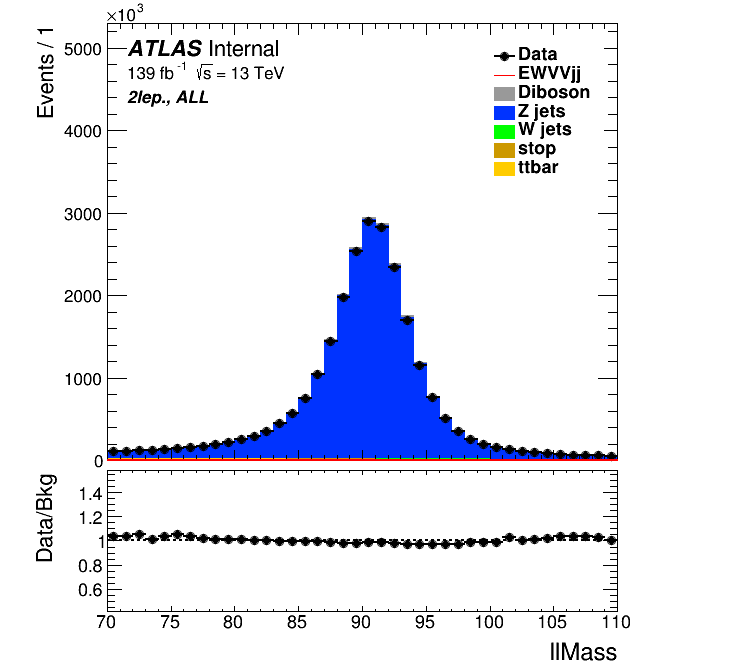
\includegraphics[width=0.5\textwidth]{figures/2lep/dataMC/C_0ptag1pfat0pjet_0ptv_ALL_llMass_Lin}
    \caption{Lepton distributions in 2-lepton channel. The events before any selections are shown. Z mass peak can be seen in $M_{ll}$ distribution.}
    \label{fig:2lepLeptons}
\end{figure}
%\section{VBS topology selection}
\subsection{Selection of the tagging jet}
It is expected for VBS process to have a pair of small-R jets in the forward-backward directions, referred to as tagging jets, in addition to the jets induced from hadronically-decaying quarks.
Requiring the tagging jets is a particular feature of the VBS process, and it helps separating signal process efficiently from the main backgrounds.
The tagging jets are selected from the small-R jets, and must not be identified as b-tagged jets to suppress the contribution of the top-quark background. 
The fJVT selection is applied to suppress the pileup jets contibutions. Tagging jet candidates are selected from the pairs of jets in opposite hemispheres, $\eta_{\operatorname{tag} j_{1}} \cdot \eta_{\operatorname{tag} j_{2}}<0$, each of which have $p_\mathrm{T} > 30~\mathrm{GeV}$ and $|\eta| < 4.5$, and the one with the highest dijet invariant mass is chosen.  
Selected tagging jets are required to have the dijet invariant mass, $m^{tag}_{jj} > 400$~GeV.
The tagging jets are selected prior to the signal jets. This order of the jet selection is optimized to maximize the signal sensitivity.
Figure~\ref{fig:Mtagjj} shows the $m^{tag}_{jj}$ distribution before selecting the analysis regions in 2-lepton channel.
As shown in the figure~\ref{fig:Mtagjj}, $m^{tag}_{jj}$ in the simulated events does not agree with data well.
The $m^{tag}_{jj}$ reweighting, which is described in Chapter~\ref{chap:modeling}, is applied before defining the analysis regions to correct the shape of the Z+jet modeling.
\begin{figure}[ht]
    \centering
    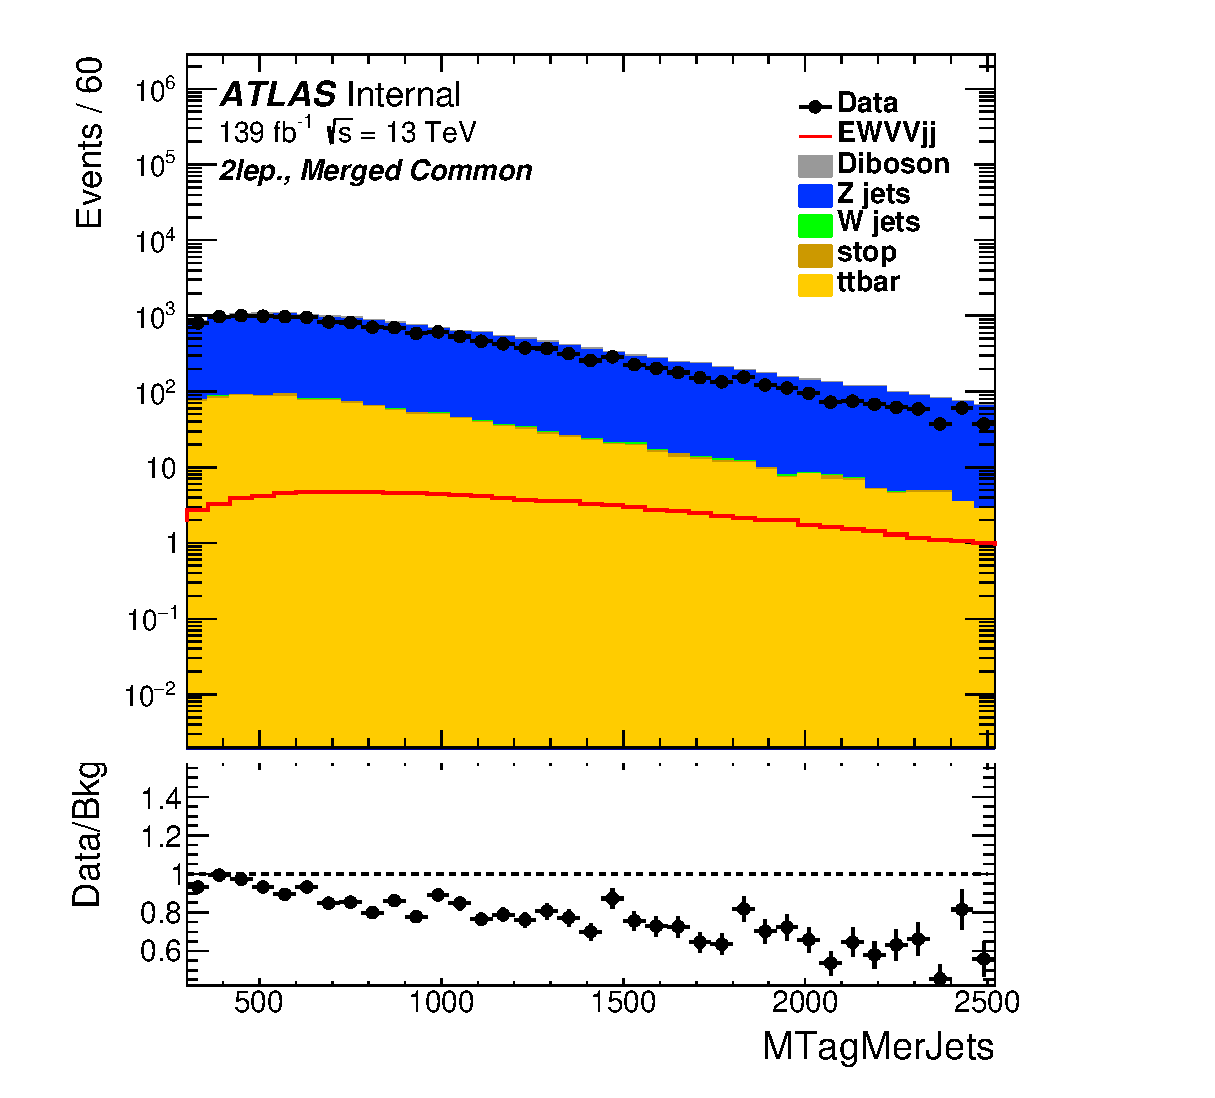
\includegraphics[width=0.48\textwidth]{figures/2lep/dataMC/C_0ptag1pfat0pjet_0ptv_MergedCommon_MTagMerJets_Log}
    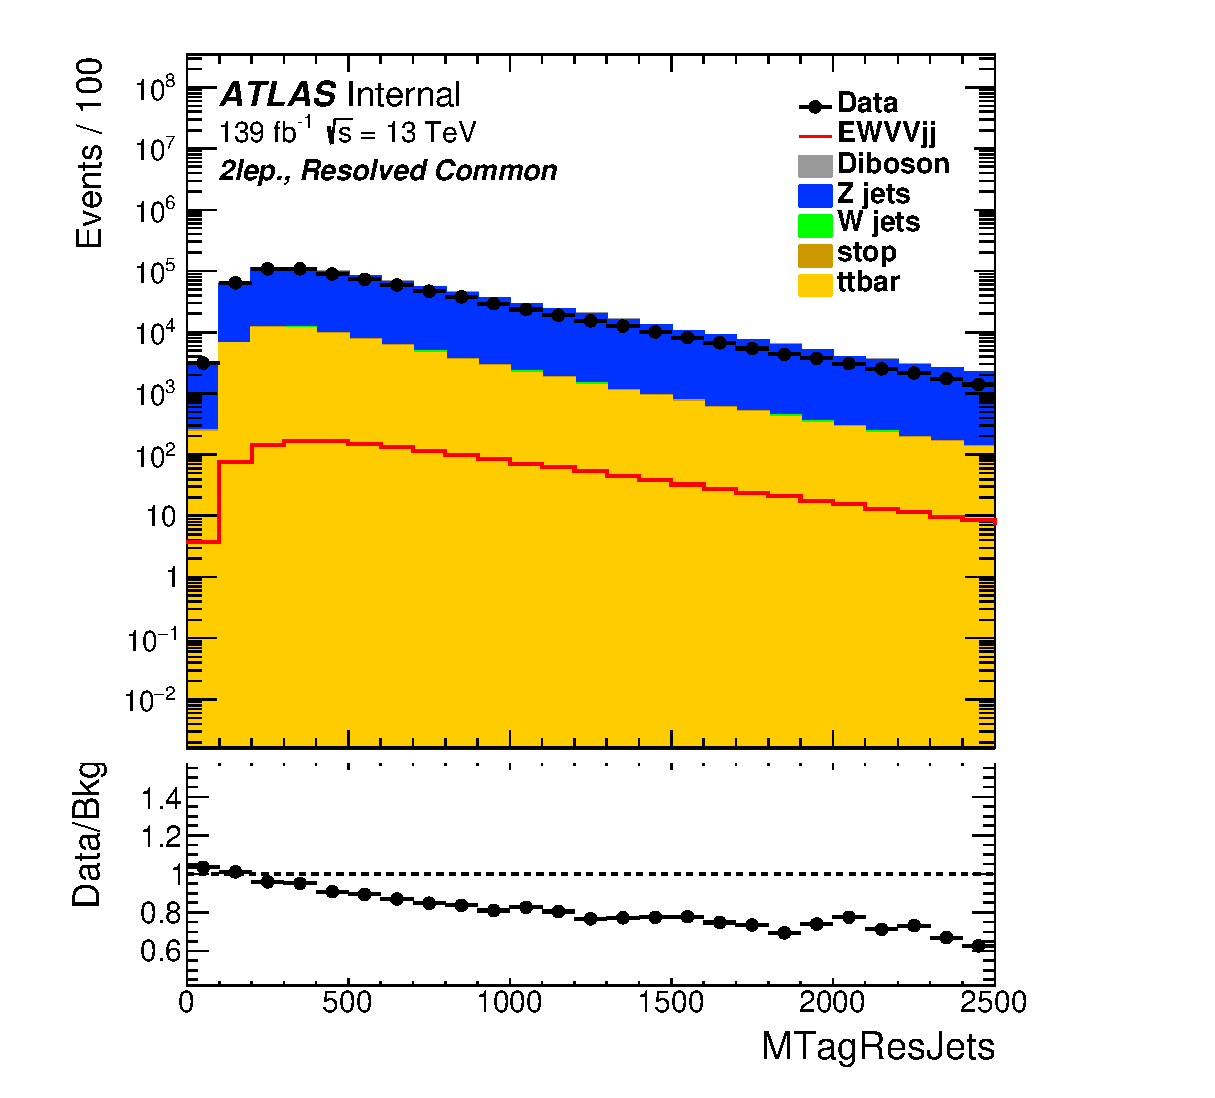
\includegraphics[width=0.48\textwidth]{figures/2lep/dataMC/C_0ptag2pjet_0ptv_ResolvedCommon_MTagResJets_Log} 
    \caption{$m^{tag}_{jj}$ distribution before defining the SRs in merged selection (left) and in resolved selection (right). The known slope due to the Z+jets modeling issue can be seen. Details are described in Chapter~\ref{chap:modeling}. $m^{tag}_{jj} > 400$GeV cut is applied to these distribution to enhance the signal sensitivity.}
    \label{fig:Mtagjj}
\end{figure}

\subsection{Selection of hadronically decaying boson}
Hadronically decaying boson ($V_{had}$) is reconstructed as a single large-R jet and a pair of small-R jets in merged selection and resolved selection, respectively. \\ \\
\noindent\textbf{\sf{Merged selection}}  \\
The leading large-R jet not overlapping with any of the tagging jets by $|\Delta R|>1.4$, to avoind the double counting of the energy deposits, is selected as the signal jet candidate (sigJ).
The sigJ is required to have a $p_{T} \geq ~200~\mathrm{GeV}$, $|\eta| < 2.0$, and not overlapping with leptons by $|\Delta R|>1.0$.

In order to select events including sigJ coming from the W/Z hadronically decay, the boson-tagger is applied. Events are further divided into subcategories depending on the result of the boson-tagger. The events passing the boson-tagger 50~\% efficiency working point is categorized in the so-called high-purity (HP) signal region (SRVBS\_HP), while those failing 50~\% working point but passing 80~\% working point are considered in the low-purity (LP) signal region (SRVBS\_LP) as shown in figure~\ref{fig:MergedRegion}. \\ \\ 

\noindent\textbf{\sf{Resolved selection}}  \\
For the bosons with the lower $p_\mathrm{T}$ ranges, the boson decays into the two well-separated jets. The two leading-$p_\mathrm{T}$ small-R jets are selected as the signal jet candidates, from the rest of the jets after tagging jets selection. 
%Leading-p$_T$ jets selection is optimized to avoid the artificial peak in the backgrounds and to get better sensitivity compared to the former jets selection, where selected two jets with invariant mass closest to the W/Z mass. 
The leading jet is required to have $p_\mathrm{T} > 40~\mathrm{GeV}$ and the subleading, $p_\mathrm{T} > 20~\mathrm{GeV}$. Their invariant mass ($m^{sig}_{jj}$) should be inside the mass window of 64 < $m^{sig}_{jj}$ < 106~GeV, near the W/Z mass. Figure~\ref{fig:MVHadResSR} shows that the reconstructed boson peak before requiring the mass window.

\begin{figure}[H]
    \centering
     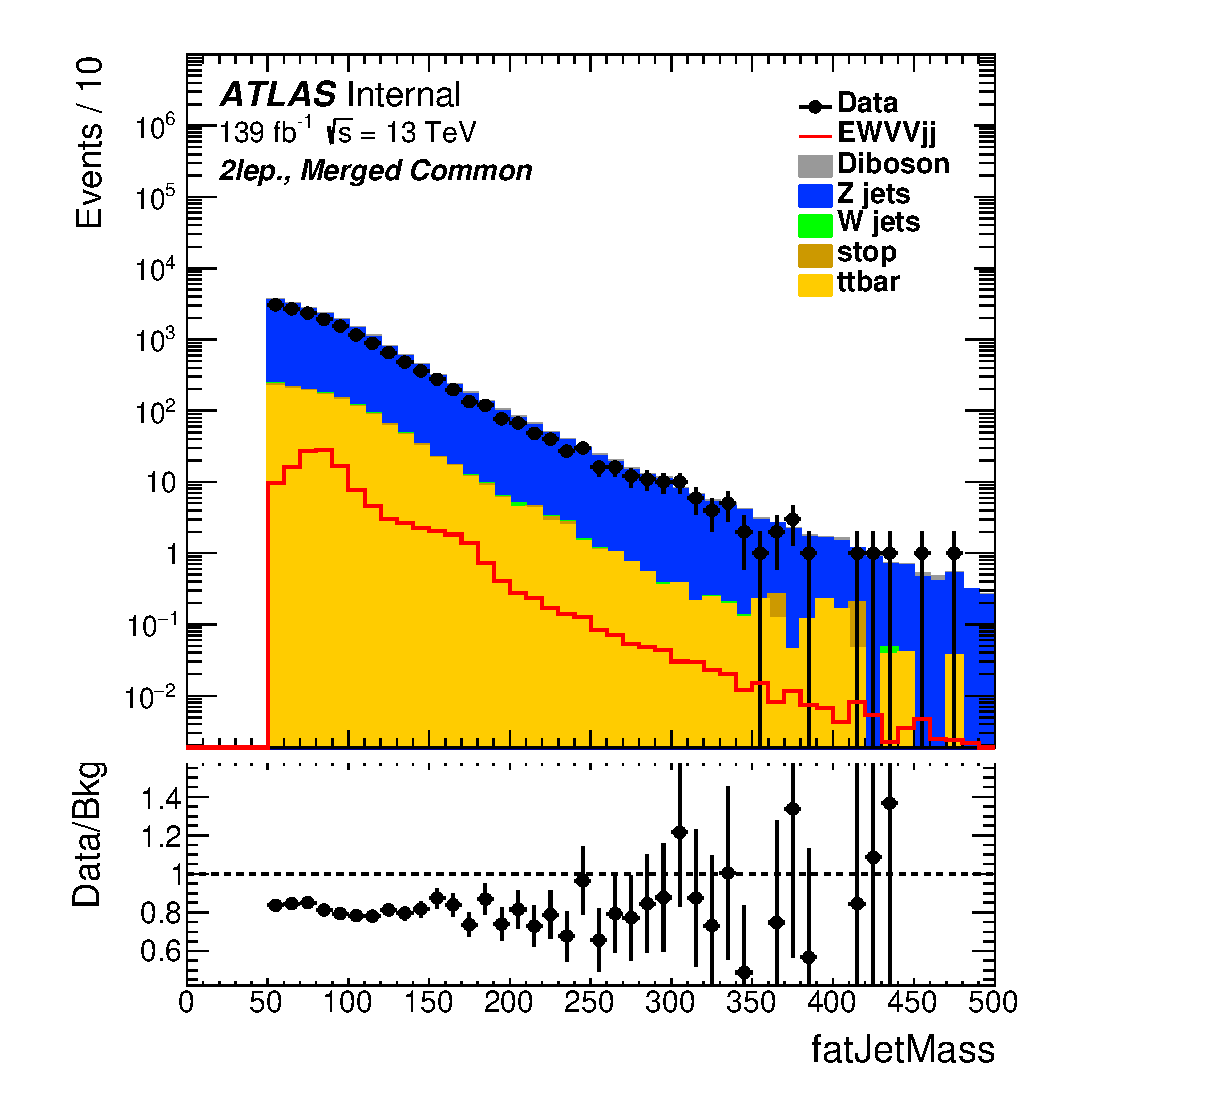
\includegraphics[width=0.48\textwidth]{figures/2lep/dataMC/C_0ptag1pfat0pjet_0ptv_MergedCommon_fatJetMass_Log} 
     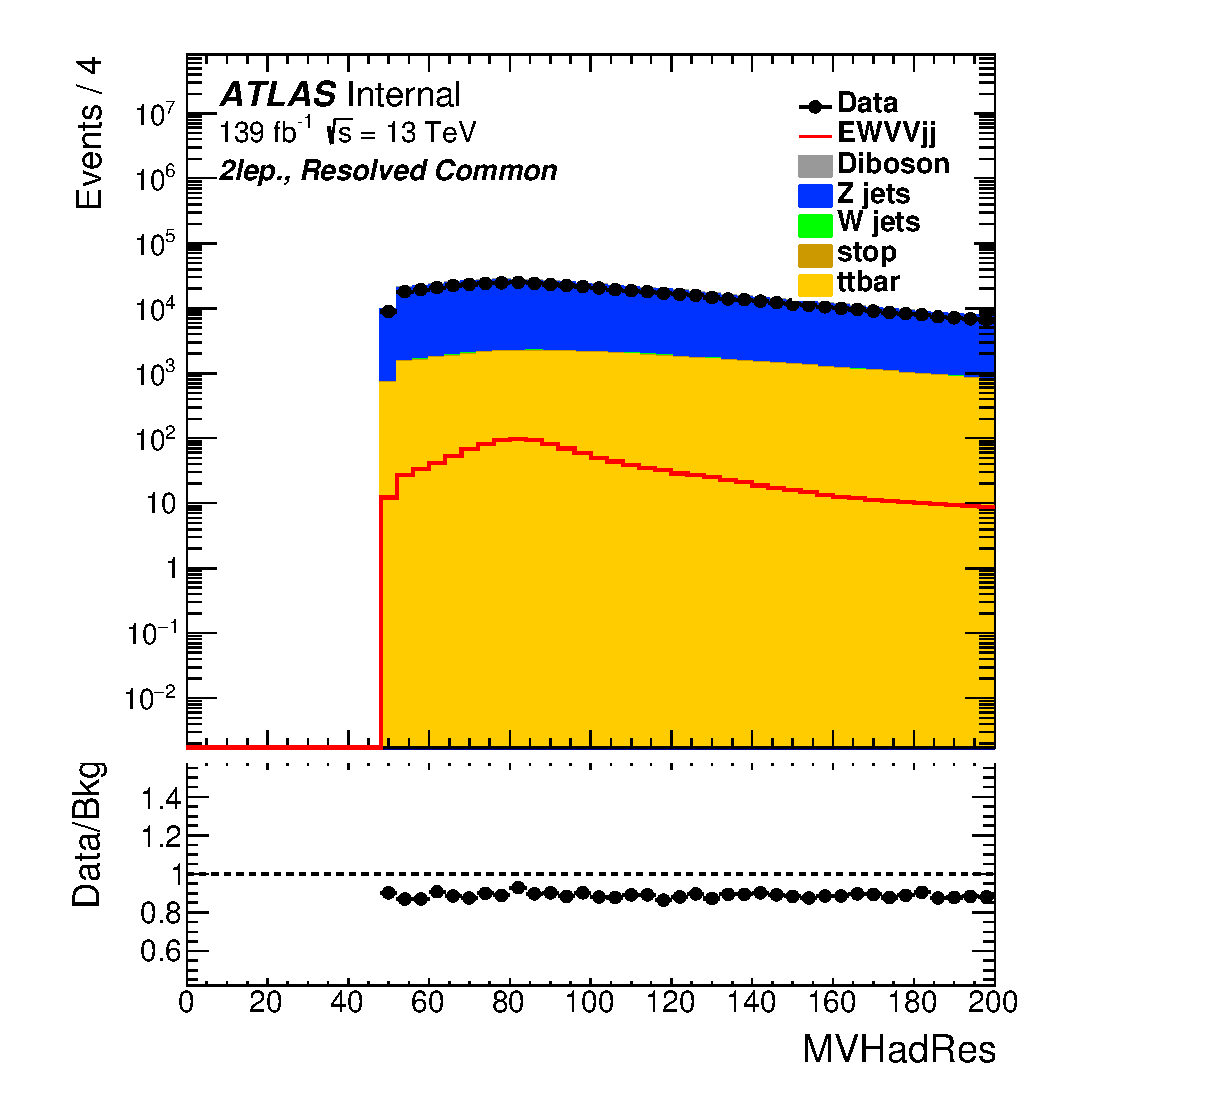
\includegraphics[width=0.48\textwidth]{figures/2lep/dataMC/C_0ptag2pjet_0ptv_ResolvedCommon_MVHadRes_Log}
    %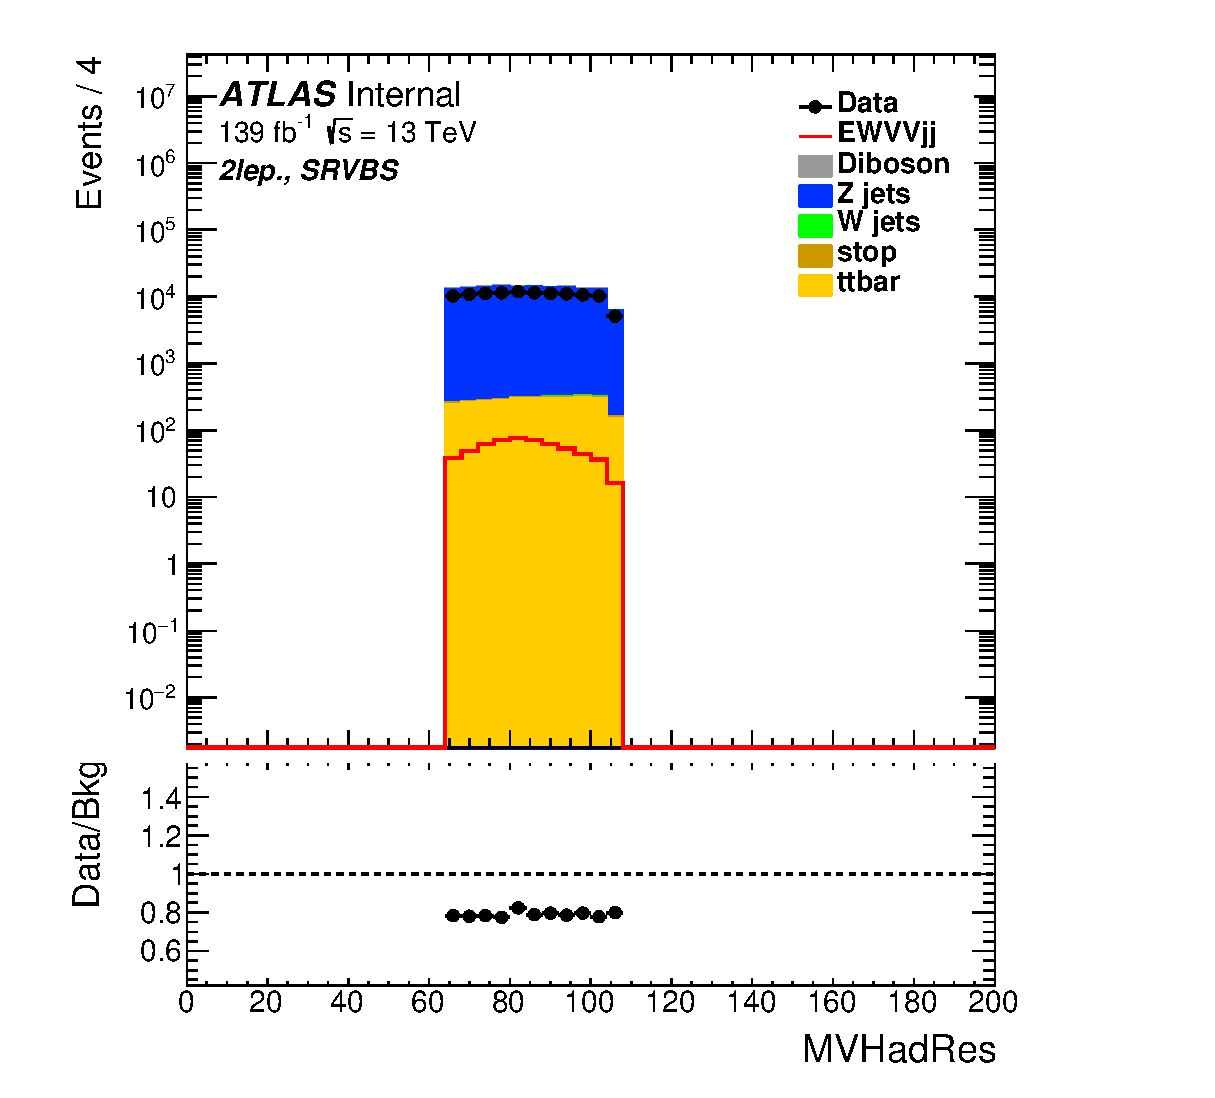
\includegraphics[width=0.4\textwidth]{figures/2lep/dataMC/C_0ptag2pjet_0ptv_SRVBS_MVHadRes_Log}
    \caption{Invariant mass of the two signal jets before requiring the boson tagger in merged region (left) and before requiring the mass window in the resolved region (right), in 2-lepton channel. 
    The second peak shown in the signal sample in merged region comes from the top contribution, for example from the process including the Wtb vertex.
    %Before the mass window cut, the $m^{tag}_{jj}$ reweighting is not applied while after mass window cut it is applied, which leads to the difference of the normalization between two plots.
    }
    \label{fig:MVHadResSR}
\end{figure}

%top mass cut
An additional cut is applied to suppress the top contributions discussed in section~\ref{subsec:sigbgMC}. A cut to the reconstructed top mass, $m_{jjj}$ > 220~GeV is applied in the resolved selection. 
The $m_{jjj}$ is derived with the two signal jets and the third jet which forms the three-jet mass, the closest to the Top mass (172.76~GeV). 
The third jet is selected from the small-R jets without the signal jets, hence can include the forward jets.
The $m_{jjj}$ for events including truth particle of top, triboson, and the others is shown in figure~\ref{fig:2leptopMass}. The reconstructed top mass peak can be seen.
\begin{figure}[H]
    \begin{center}
      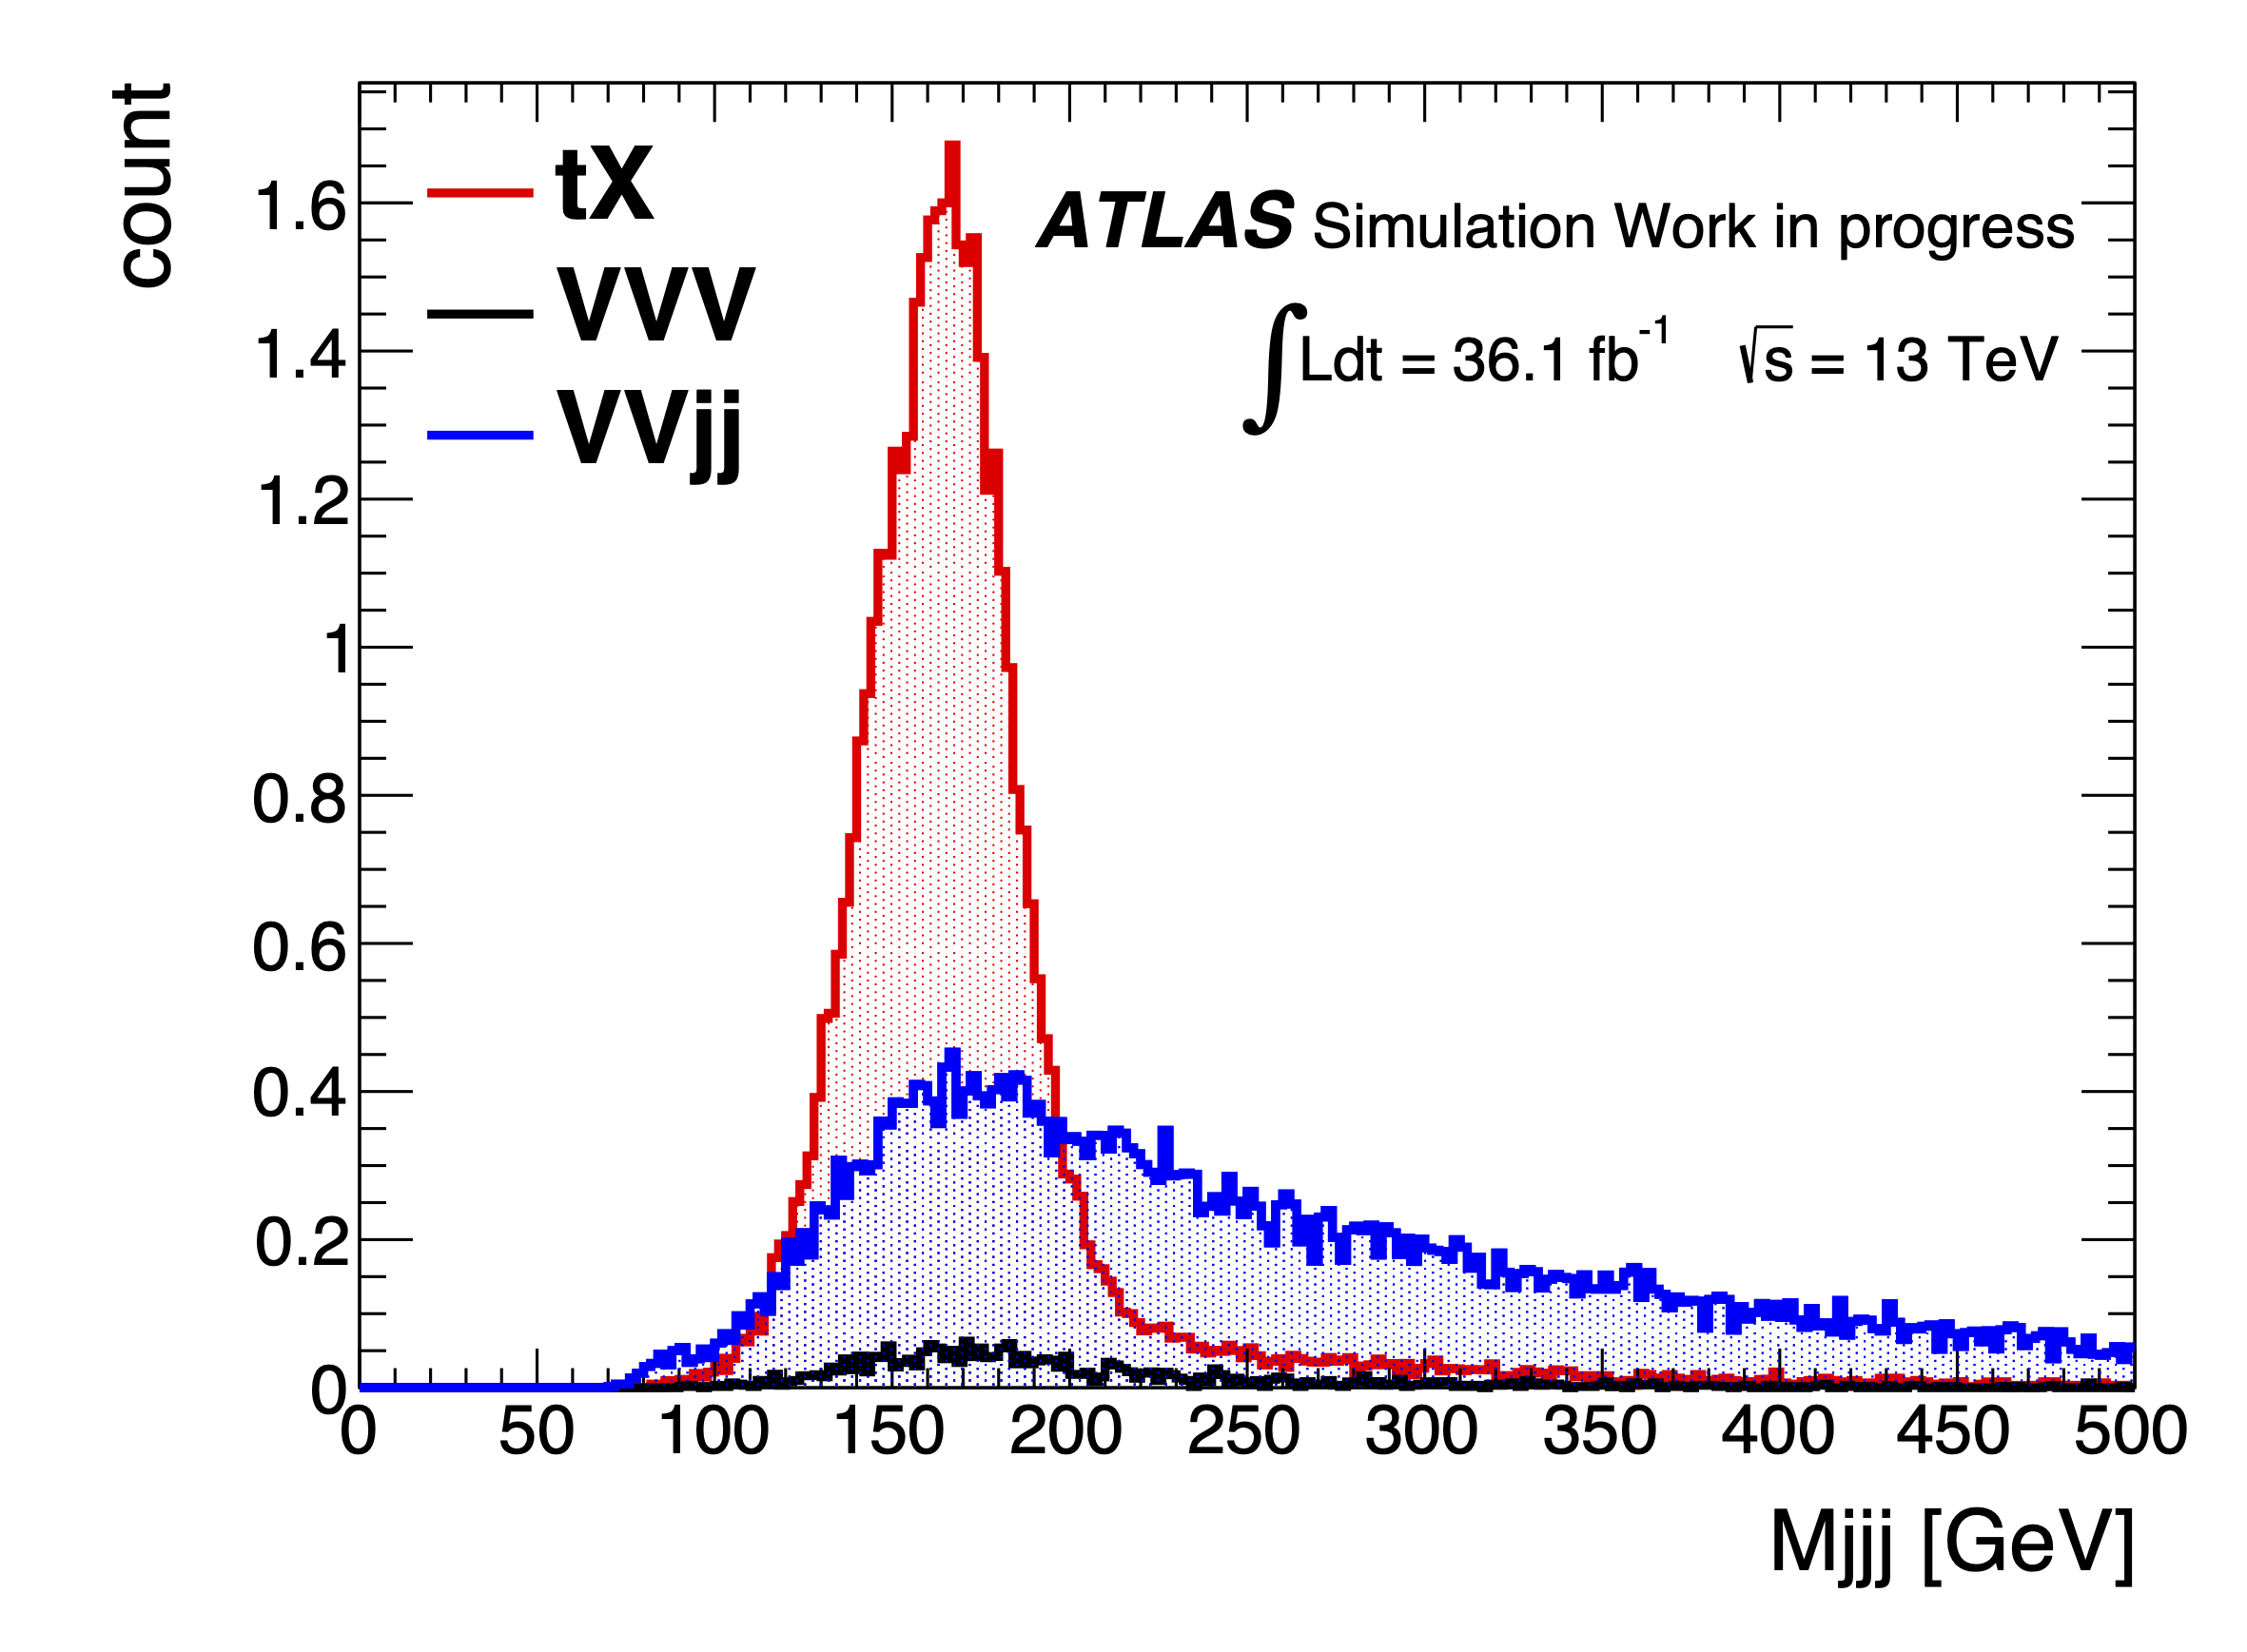
\includegraphics[width=0.48\textwidth]{figures/2lep/topMass/WZjjtopMasspeak}
      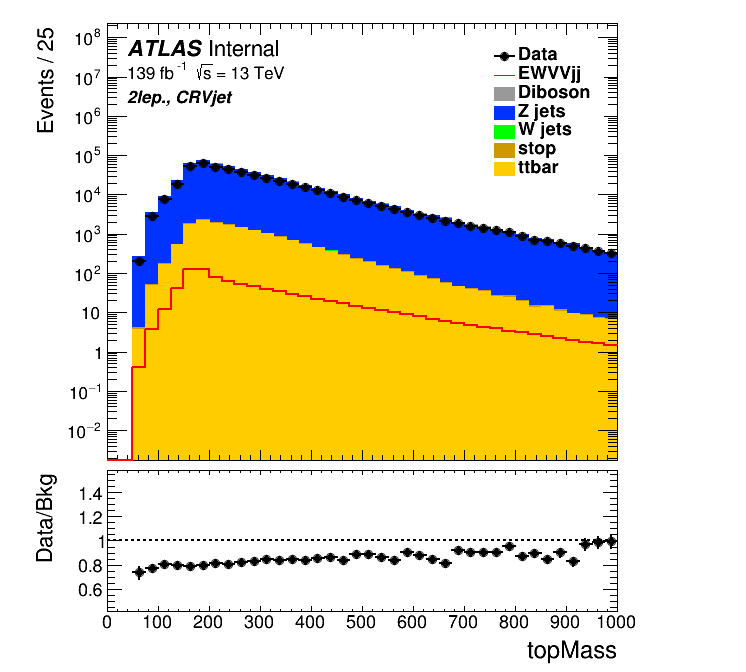
\includegraphics[width=0.48\textwidth]{figures/2lep/dataMC/C_0ptag2pjet_0ptv_CRVjet_topMass_Log}
        \caption{ Mass of 3 jets in the 2-lepton channel resolved signal region with events including top (tX, in red), 3 bosons (VV, in black), and others, which is VBS-like events (VVjj, in blue). (left) The modeling plot in resolved control region is also shown. (right)}
        \label{fig:2leptopMass}
    \end{center}
\end{figure}
This top-mass cut can reduce the top contributions, as shown in Table~\ref{fig:TruthTop2LepPurity} in resolved selection, therefore the resolved signal region (denoted as SRVBS\_Tight) is defined with this additional cut to get more VBS-like phase space. In merged selection top-mass can be defined in the similar manner, $m_{Jj}$, by the invariant mass of the large-R signal jet and the additional jet which make the closest invariant mass to the top mass. 
However, top contribution is already small without the top mass cut, after the event selections above, hence this cut is not added to the merged selection.
\begin{figure}[H]
    \centering
    \resizebox{0.95\textwidth}{!}{
    \begin{tabular}{|c||c|c|c|c|}
         \hline
                        & SRVBS (resolved) & VBS enhanced (resolved) & SRVBS (merged) & VBS enhanced (merged) \\ \hline
        Truth Top       & 0.48             & 0.14                    & 0.14           & 0.10                  \\ \hline
        Truth VVV       & 0.03             & 0.03                    & 0.08           & 0.08                  \\ \hline
        Truth VBS       & 0.49             & 0.83                    & 0.78           & 0.82                  \\ \hline
    \end{tabular}
        }
        \caption{Fraction of event yields for 2lepton channel. The truth information is used to know if the event includes each contributions. Only EWWZjj events are checked here since there are no Top contributions in EWZZjj events.}
        \label{fig:TruthTop2LepPurity}
\end{figure}

%\subsection{Selection of analysis regions}
\subsection{Control region definitions}
%The signal regions (SR) are defined each for merged (SRVBS\_HP, SRVBS\_LP) and resolved (SRVBS\_Tight) selection, according to the selection of the hadronically decaying boson candidates. All selections applied to define the SRs in each lepton channel are listed in the table in section~\ref{sec:sumES}.
The control region (CR) is defined to estimate the normalization of the main backgrounds and apply it in the signal region. 
CRs should be defined in a similar way as the SRs so that the 
%background modeling does not change when moving
uncertainty on the extrapolation from CRs to SRs is minimized.
It is defined by inverting one of the cuts to define merged and resolved categories, with keeping the other cuts to be the same as the SRs.
%the definitions of 
%the SRs, with the common event selections up to the definition of the SRs.
The dedicated CRs to the V+jets and t$\bar{\mathrm{t}}$ background events are defined in this analysis. \\ \\

\noindent\textbf{\sf{V+jets CR}}  \\
There are separate CRs for V+jet in merged and resolved categories (V is Z/W for 0-lepton, W for 1-lepton, Z for 2-lepton channel) since they have the different phase spaces and possible mismodeling of the cross section depending on the mass.
%merged and resolved CR for 
Merged V+jets CR is defined by requiring events to fail boson tagger 80~\% efficiency working point. 
Merged CR and SR definition is shown in the Figure~\ref{fig:MergedRegion}.
\begin{figure}[H]
    \centering
    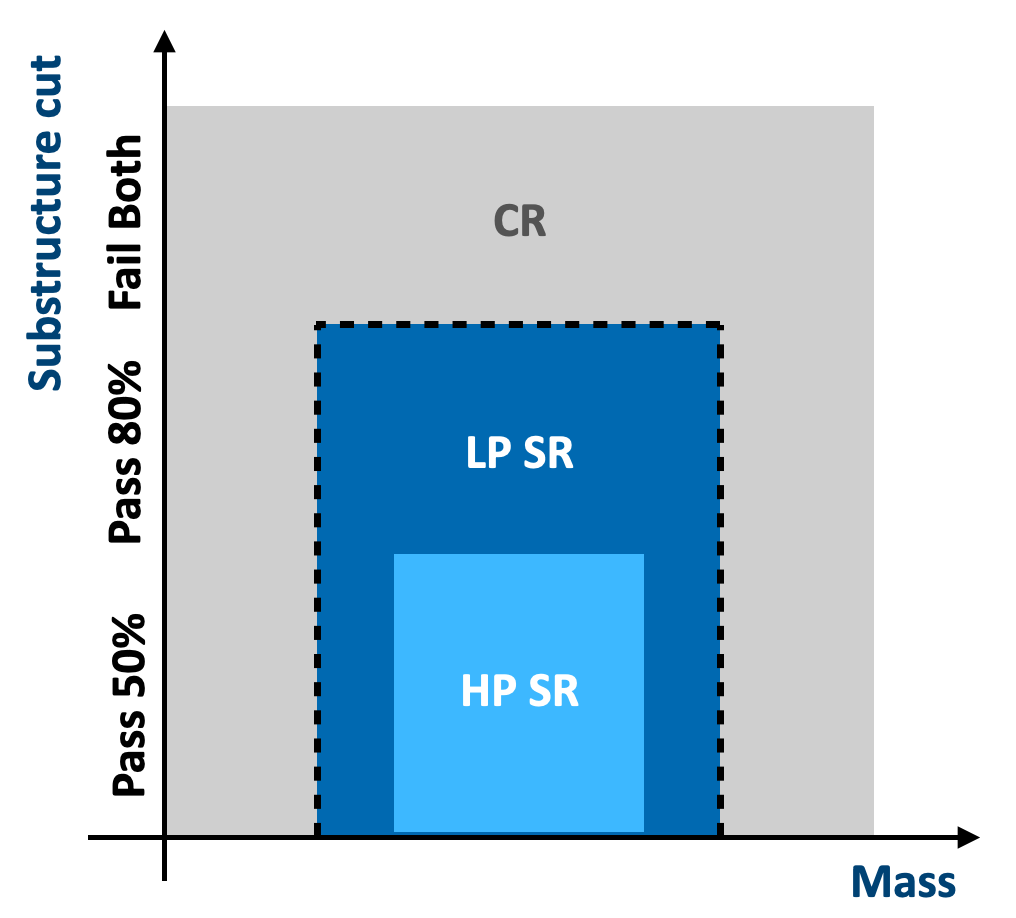
\includegraphics[width=0.4\textwidth]{figures/MergedRegion}
    \caption{The selection of the merged SR and CR are shown. The CR definition is what was changed from the previous round of the analysis, in order to fulfill the requirement to derive the scale factors.}
    \label{fig:MergedRegion}
\end{figure}
The normalization of the V+jets background is estimated in merged CR, and is propagated to the SR by assuming the efficiency of the boson tagger is well modeled by the simulation.
The possible data-to-MC disagreement of the efficiency and its uncertainty is estimated using dedicated data samples independent of this study. 
%from the other analysis~\cite{ATL-PHYS-PUB-2015-053}.
%The 50~\% working point boson tagging efficiency scale factor, denoted SF$_{\mathrm{eff}, 50\%}$ here, is applied to the SRVBS\_HP. 
%For the SRVBS\_LP, considering the correlation between 50~\% and 80~\% working point,
%\begin{equation*}
%\mathrm{SF}_{\mathrm{eff}, \mathrm{LP}}  = \frac{\epsilon_{80\%}~\mathrm{SF}_{\mathrm{eff}, 80\%} - \epsilon_{50\%}~\mathrm{SF}_{\mathrm{eff}, %50\%}}{\epsilon_{80\%} - \epsilon_{50\%}}
%\end{equation*}
%is applied.

In the resolved V+jets CR, events are selected by reverting the mass window cut, which should satisfy $50<m_{i i}<64 ~\mathrm{GeV}$, or $m_{i i}>106 ~\mathrm{GeV}$. 
Figure~\ref{fig:CRVjet} shows the mass of the reconstructed boson in CRs. The Z+jets background has continuous mass distributions in CR and SR hence its normalization can be estimated from mass-sideband in CR, while signal has a significant peak in SR as can be seen in figure~\ref{fig:MVHadResSR}.

\begin{figure}[H]
    \centering
    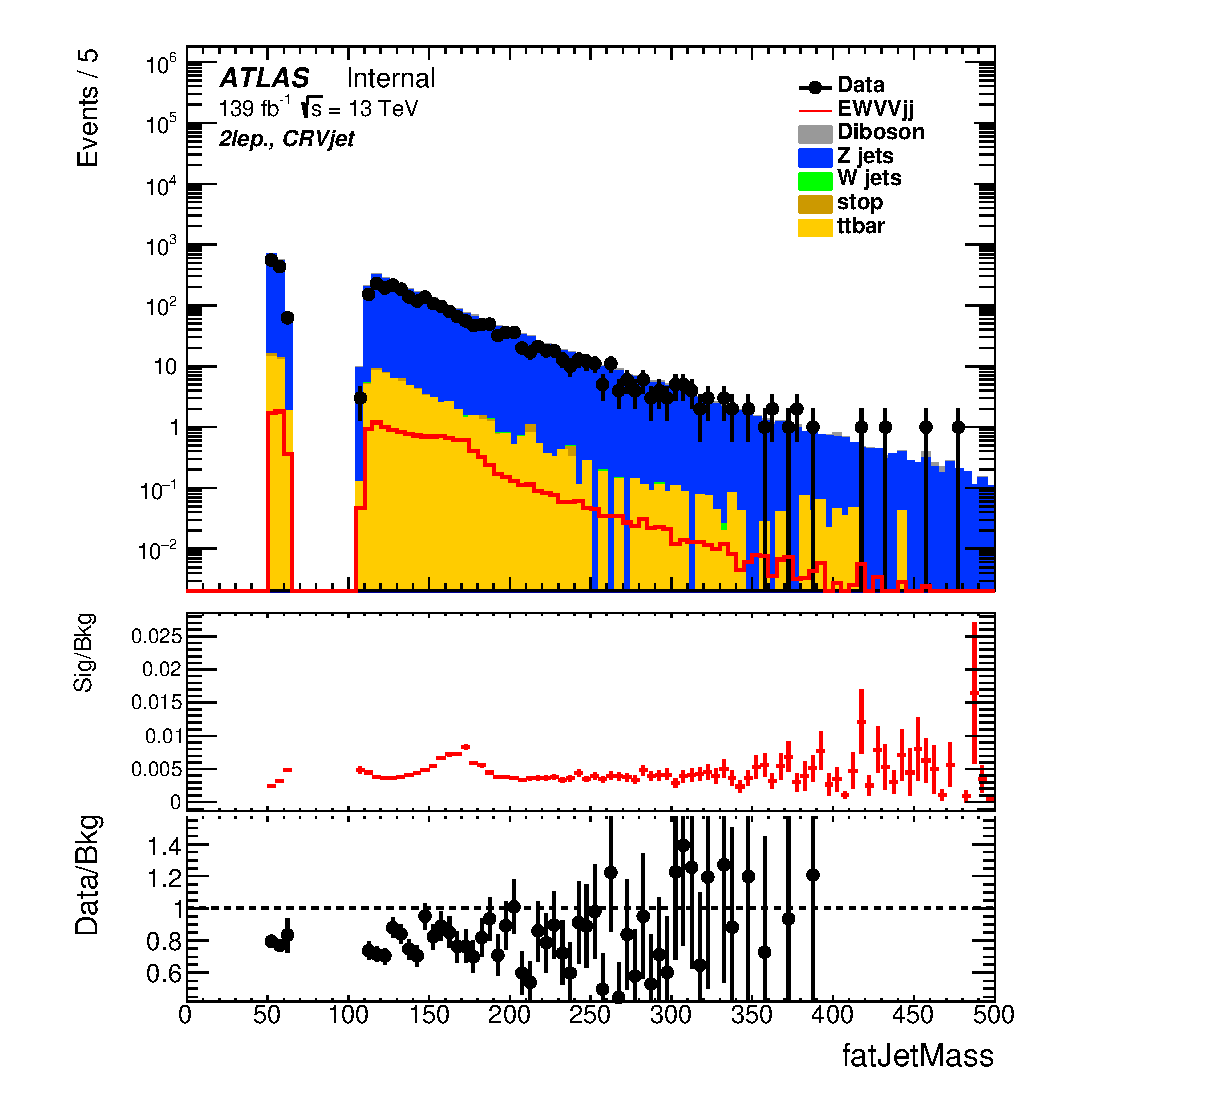
\includegraphics[width=0.48\textwidth]{figures/2lep/dataMC/C_0ptag1pfat0pjet_0ptv_CRVjet_fatJetMass_Log}
    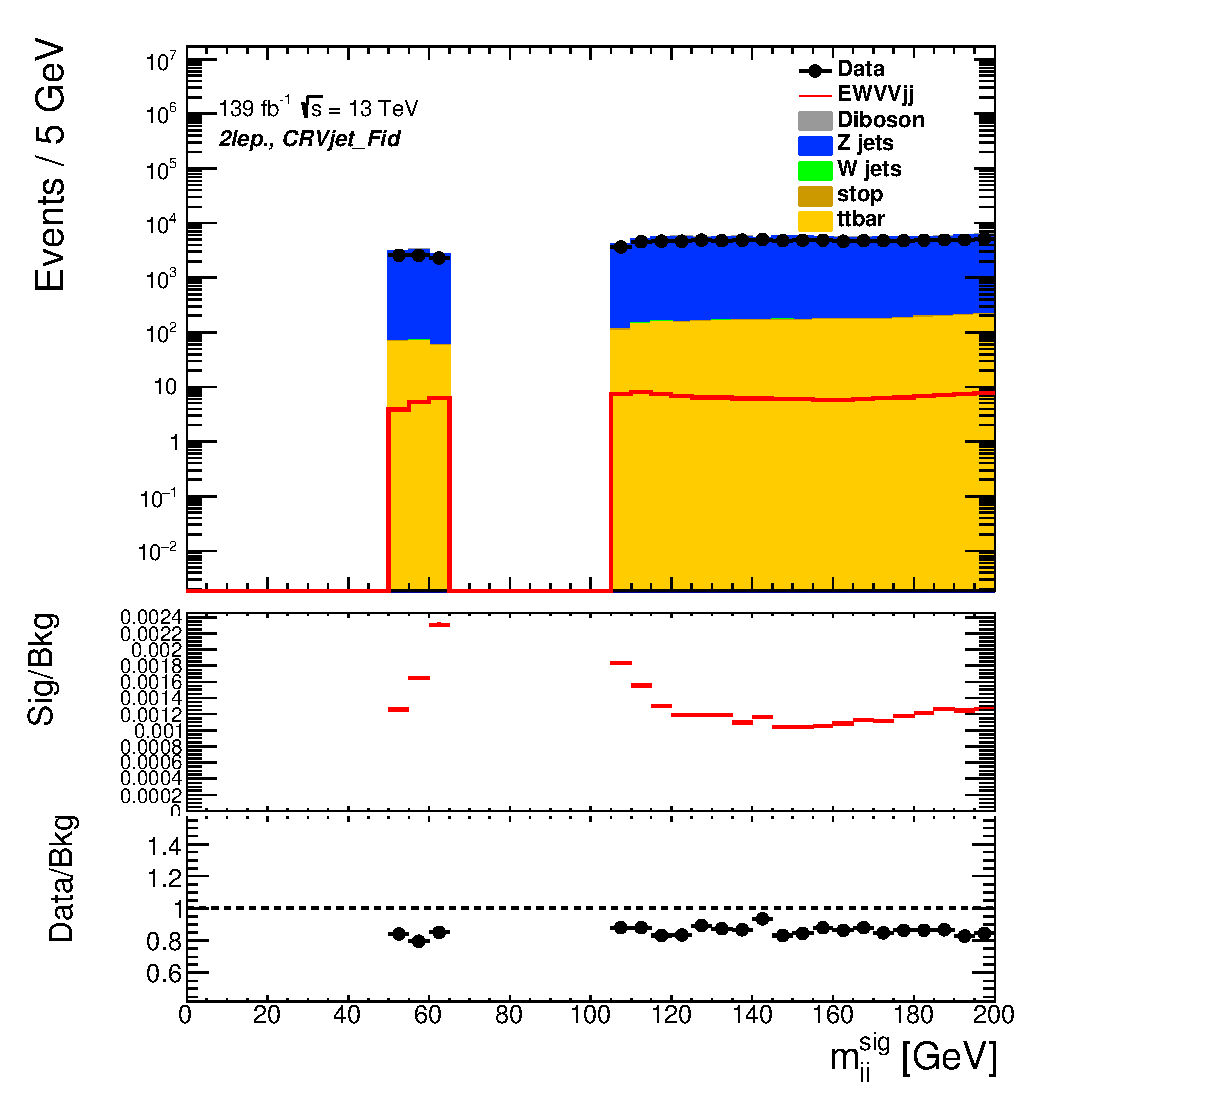
\includegraphics[width=0.48\textwidth]{figures/2lep/dataMC/C_0ptag2pjet_0ptv_CRVjet_Fid_MVHadRes_Log}
    \caption{Mass of reconstructed boson in the resolved CR}
    \label{fig:CRVjet}
\end{figure}

In the intermediate $p_\mathrm{T}$ range, hadronically decaying boson can be reconstructed by both merged and resolved selections.
The order of the event selection is optimized to increase the sensitivity after the combination of merged and resolved analyses. 
Event is first analyzed in the merged selection, and if it does not satisfy the selection cut for that, it is reanalyzed in the resolved category.
The event selection is performed subsequently in the order shown in the diagram in figure~\ref{fig:order}.
\begin{figure}[H]
    \centering
    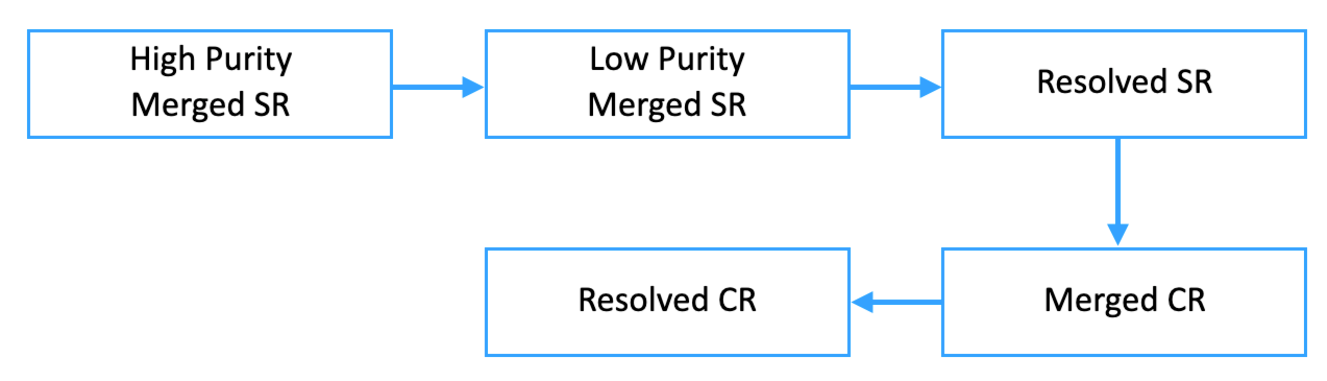
\includegraphics[width=0.65\textwidth]{figures/order}
    \caption{The order of defining the SR and the CR. The merged SR are defined at first, and the events failed the merged SR selections goes to the selection of the resolved SR, therefore there are no overlapped events within several SR and CRs.}
    \label{fig:order}
\end{figure}

%%%%%%%% end of the section
%%??? for boson tagger scale factor
%The 50~\% working point (WP) $W/Z$-tagging scale factor is applied for the HP SR, and a custom scale factor is defined for the LP SR:
%\begin{equation}
%S F_{L P}=\frac{\epsilon_{loose} S F_{eff, loose}-\epsilon_{tight} S F_{eff, tight}}{\epsilon_{loose}-\epsilon_{tight}}
%\end{equation}
%where "loose" refers to the 80\% WP and "tight" refers to the 50\% WP.
%The boson-tagger is optimized to maximize the sensitivity to the longitudinally-polarized $W/Z$ bosons. 
%The previous study showed that the HPSR is not so sensitive to the fully-transversed aQGC signals, which makes us to keep the LPSR for the aQGC searches. 
%In the merged CR, the inefficiency scale factors $SF_{ineff,loose}$ calaculated for the 80\% working point tagger are applied:
%\begin{equation}
%S F_{i n e f f}=\frac{1-\epsilon \times S F_{e f f}}{1-\epsilon}
%\end{equation}
%where $\epsilon$ is the efficiency estimated in ttbat events for signal and $\gamma$+jet and multi-jet events for background.
%%%%%%


%top CR
\noindent\textbf{\sf{Top CR}}  \\
Top CR is used to constraint the normalization of the t$\bar{\mathrm{t}}$ background. It exists only in 1-lepton channel, where selected events contain plenty of t$\bar{\mathrm{t}}$ background. 
It is defined by requiring at least one b-tagged jet instead of b-veto. Requiring of the b-tagging is applied after the hadronically decaying boson selection, therefore there is three Top CRs according to the SRs: Resolved Top CR, Merged HP CR, Merged LP CR.

\section{Summary of the event selections}
\label{sec:sumES}
The summary of the whole event selection applied in each channel is shown here in the Table~\ref{tab:0lep_merged}-\ref{tab:0lep_resolved} (0-lepton), \ref{tab:1lep_merged}-\ref{tab:1lep_resolved} (1-lepton), \ref{tab:2lep_merged}-\ref{tab:2lep_resolved} (2-lepton).

%%% 0-lepton channel
\begin{table}[H]
\small
\begin{center}
\resizebox{0.8\textwidth}{!}{
\begin{tabular}{|l|l|c|c|c|}
\hline
\multicolumn{2}{|l|}{\multirow{2}{*}{Selection}} & \multicolumn{2}{c|}{SR}  &  $V$ CR \\
\cline{3-5}
\multicolumn{2}{|l|}{} & HP & LP &  \\
\hline
\multirow{3}{*}{$Z \to \nu\nu$}  &  Number of Loose leptons & \multicolumn{3}{c|}{0} \\
\cline{2-5}
    & \met                                     & \multicolumn{3}{c|}{ > 200 GeV }                  \\
\cline{2-5}
    & \mpt                                     & \multicolumn{3}{c|}{ > 50 GeV}                    \\
\hline

\multirow{3}{*}{anti-QCD}  & min($\Delta\Phi$(\met,small-R jets))     & \multicolumn{3}{c|}{ $> \pi/6$} \\
\cline{2-5}
    & $\Delta\Phi$(\met,\mpt)                  & \multicolumn{3}{c|}{ $< \pi/2$}                   \\
\cline{2-5}
    & $\Delta\phi(\met, Sig-J)$                & \multicolumn{3}{c|}{ $> \pi/9$}                   \\
\hline
\multirow{3}{*}{VBS jets candidates} & Leading Tag jet \pt & \multicolumn{3}{c|}{ $>30\,\GeV$ } \\
\cline{2-5}
                          & Subleading Tag jet \pt & \multicolumn{3}{c|}{ $>30\,\GeV$ }\\
\cline{2-5}
                          & $m_{jj}$ & \multicolumn{3}{c|}{ $> 400 \GeV$ } \\
\hline
\multirow{2}{*}{$W/Z \to J$} & Num of large-R jets & \multicolumn{3}{c|}{$\geq 1$} \\
\cline{2-5}
& 3-Var Tagger & pass50WP & pass80WP \&\& !pass50WP & fail80WP \\
\hline
\end{tabular}
}
\end{center}
\caption{A summary of regions event selection for \zlep channel in the merged regime.}
\label{tab:0lep_merged}
\end{table}

\begin{table}[H]
\small
\begin{center}
\resizebox{0.8\textwidth}{!}{
\begin{tabular}{|l|l|c|c|}
\hline
\multicolumn{2}{|l|}{Selection} & SR  & $V$ CR \\
\hline
\multirow{3}{*}{$Z \to \nu\nu$}  &  Number of Loose leptons & \multicolumn{2}{c|}{0} \\
\cline{2-4}
    & \met                                     & \multicolumn{2}{c|}{ > 200 GeV }                  \\
\cline{2-4}
    & \mpt                                     & \multicolumn{2}{c|}{ > 50 GeV}                    \\
\hline

\multirow{3}{*}{anti-QCD}  & min($\Delta\Phi$(\met,small-R jets))     & \multicolumn{2}{c|}{ $> \pi/6$} \\
\cline{2-4}
    & $\Delta\Phi$(\met,\mpt)                  & \multicolumn{2}{c|}{ $< \pi/2$}                   \\
\cline{2-4}
    & $\Delta\phi(\met, Sig-J)$                & \multicolumn{2}{c|}{ $> \pi/9$}                   \\
\hline
\multirow{3}{*}{VBS jets candidates} & Leading Tag jet \pt & \multicolumn{2}{c|}{ $>30\,\GeV$ } \\
\cline{2-4}
                          & Subleading Tag jet \pt & \multicolumn{2}{c|}{ $>30\,\GeV$ }\\
\cline{2-4}
                          & $m_{jj}$ & \multicolumn{2}{c|}{ $> 400 \GeV$ } \\
\hline
\multirow{4}{*}{$W/Z \to jj$} & Number of small-R jets & \multicolumn{2}{c|}{$\geq 4$} \\
\cline{2-4}
              & Leading signal jet \pt & \multicolumn{2}{c|}{ $>40\,\GeV$ }\\
\cline{2-4}
              & Subleading signal jet \pt & \multicolumn{2}{c|}{ $>20\,\GeV$ }\\
\cline{2-4}
              &$Z \to q\bar{q}$ and $W \to q\bar{q}$     &   $64 < m_{jj} < 106 \gev$ & $50<m_{jj}<64 \,GeV$ or $m_{jj}>106$ \\
\hline
VBS enhancing & $m_{jjj}$ & \multicolumn{2}{c|}{ $>220$~GeV} \\
\hline
\end{tabular}
}
\end{center}
\caption{A summary of regions event selection for \zlep channel in the resolved regime.}
\label{tab:0lep_resolved}
\end{table}

%%% 1-lepton channel
\begin{table}[H]
\begin{center}
\resizebox{0.95\textwidth}{!}{
\begin{tabular}{|l|l|c|c|c|c|c|}
\hline
\multicolumn{2}{|l|}{\multirow{2}{*}{Selection}} & \multicolumn{2}{c|}{SR}  &  $W$ CR (WR)  & \multicolumn{2}{c|}{$t\bar{t}$ CR (TR)} \\
\cline{3-7}
\multicolumn{2}{|l|}{} & HP & LP & incl & HP & LP \\
\hline
\multirow{4}{*}{$W\rightarrow \ell\nu$} & Num of Tight leptons & \multicolumn{5}{c|}{ 1 } \\
\cline{2-7}
&Num of Loose (!Tight) leptons & \multicolumn{5}{c|}{ 0 }  \\
\cline{2-7}
&\vphantom{\Large B} \met & \multicolumn{5}{c|}{ $>80\,\GeV$ } \\
\cline{2-7}
&$\pt(\ell)$ & \multicolumn{5}{c|}{ $>30\,\GeV$ } \\
\hline
\multirow{3}{*}{VBS jets candidates} & Leading Tag jet \pt & \multicolumn{5}{c|}{ $>30\,\GeV$ } \\
\cline{2-7}
                          & Subleading Tag jet \pt & \multicolumn{5}{c|}{ $>30\,\GeV$ }\\
\cline{2-7}
                          & $m_{jj}$ & \multicolumn{5}{c|}{ $> 400 \GeV$ } \\
\hline
\multirow{2}{*}{$W/Z\rightarrow J$} & Num of large-$R$ jets & \multicolumn{5}{c|}{ $\geq 1$ } \\
\cline{2-7}
& 3-Var Tagger & pass50WP & pass80WP \&\& !pass50WP & fail80WP & pass50WP & pass80WP \&\& !pass50WP \\
%& \vphantom{\Large B} $D_2/n_{Tracks}$ cut & pass & fail & pass & fail & pass & fail \\
%\cline{2-8}
%& $W/Z$ mass window cut & pass & pass & fail & fail & pass & pass\\
\hline
Top veto & Num of $b$-tagged jets outside of large-R jet & \multicolumn{3}{c|}{0} & \multicolumn{2}{c|}{$\geq 1$} \\
\hline
\end{tabular}
}
\end{center}
\caption{A summary of regions event selection for \olep channel in the merged regime.}
\label{tab:1lep_merged}
\end{table}
\begin{table}[H]
\begin{center}
\resizebox{0.95\textwidth}{!}{
\begin{tabular}{|l|l|c|c|c|}
\hline
\multicolumn{2}{|l|}{Selection} & SR & $W$ CR (WR) & \ttbar CR (TR) \\
\hline
\multirow{4}{*}{$W\rightarrow \ell\nu$ } & Number of Tight leptons & \multicolumn{3}{c|}{ 1 } \\
\cline{2-5}
&Number of Loose (!Tight) leptons & \multicolumn{3}{c|}{ 0 }  \\
\cline{2-5}
&\met & \multicolumn{3}{c|}{ $>80\,\GeV$ } \\
\cline{2-5}
&$\pt(\ell)$ & \multicolumn{3}{c|}{ $>30\,\GeV$ } \\
\hline
\multirow{3}{*}{VBS jets candidates} & Leading Tag jet \pt & \multicolumn{3}{c|}{ $>30\,\GeV$ } \\
\cline{2-5}
                          & Subleading Tag jet \pt & \multicolumn{3}{c|}{ $>30\,\GeV$ }\\
\cline{2-5}
                          & $m_{jj}$ & \multicolumn{3}{c|}{ $> 400 \GeV$ } \\
\hline
\multirow{4}{*}{$W/Z\rightarrow jj$ } & Number of small-R jets & \multicolumn{3}{c|}{ $\geq 4$ } \\ %$\geq 2$ & $\geq 2$ & $\geq 2$  \\
\cline{2-5}
& Leading jet \pt & \multicolumn{3}{c|}{ $>40$~GeV}\\
\cline{2-5}
& Subleading jet \pt & \multicolumn{3}{c|}{ $>20$~GeV}\\
\cline{2-5}
 &$Z \to q\bar{q}$ and $W \to q\bar{q}$     &   $64 < m_{jj} < 106 \gev$ & $50<m_{jj}<64 \,GeV$ or $m_{jj}>106$ & $64 < m_{jj} < 106 \gev$ \\
\hline
Top veto &  Number of additional $b$-tagged jets & \multicolumn{2}{c|}{0} & $\geq 1$ \\
\hline
VBS enhancing & $m_{jjj}$ & \multicolumn{3}{c|}{ $>220$~GeV} \\
\hline
\end{tabular}
}
\end{center}
 \caption{A summary of regions event selection for \olep~channel in the resolved regime.}
 \label{tab:1lep_resolved}
\end{table}

%%% 2-leptons channel
\begin{table}[H]
\small
\begin{center}
\resizebox{0.8\textwidth}{!}{
\begin{tabular}{|l|l|c|c|c|}
\hline
\multicolumn{2}{|l|}{\multirow{2}{*}{Selection}} & \multicolumn{2}{c|}{SR}  &  $Z$ CR \\
\cline{3-5}
\multicolumn{2}{|l|}{} & HP & LP & incl \\
\hline
\multirow{6}{*}{$Z \to \ell\ell$}  &  Number of Loose leptons & \multicolumn{3}{c|}{2} \\
\cline{2-5}
                          & Same flavor &  \multicolumn{3}{c|}{yes} \\
\cline{2-5}
                          & Leading lepton \pt  & \multicolumn{3}{c|}{$>27\,\GeV$} \\
\cline{2-5}
                          & Subleading lepton \pt  & \multicolumn{3}{c|}{$>27\,\GeV$} \\
\cline{2-5}
                          & \multirow{2}{*}{dilepton invariant mass} & \multicolumn{3}{c|}{$ 83 < m_{ee} < 99 \gev$} \\
                          &  & \multicolumn{3}{c|}{$-0.01170\ptll+85.63 < m_{\mu\mu} < 0.01850\ptll+94.00 \gev$} \\
\cline{2-5}
                          & Opposite sign &  \multicolumn{3}{c|}{For $\mu\mu$ channel only} \\
\hline
\multirow{3}{*}{VBS jets candidates} & Leading Tag jet \pt & \multicolumn{3}{c|}{ $>30\,\GeV$ } \\
\cline{2-5}
                          & Subleading Tag jet \pt & \multicolumn{3}{c|}{ $>30\,\GeV$ }\\
\cline{2-5}
                          & $m_{jj}$ & \multicolumn{3}{c|}{ $> 400 \GeV$ } \\
\hline
\multirow{2}{*}{$W/Z \to J$} & Num of large-R jets & \multicolumn{3}{c|}{$\geq 1$} \\
\cline{2-5}
& 3-Var Tagger & pass50WP & pass80WP \&\& !pass50WP & fail80WP \\
\hline
\end{tabular}
}
\end{center}
\caption{A summary of regions event selection for 2-lepton channel in the merged selection.}
\label{tab:2lep_merged}
\end{table}

\begin{table}[H]
\small
\begin{center}
\resizebox{0.8\textwidth}{!}{
\begin{tabular}{|l|l|c|c|}
\hline
\multicolumn{2}{|l|}{Selection} & SR  & $Z$ CR \\
\hline
\multirow{6}{*}{$Z \to \ell\ell$}  &  Number of Loose leptons & \multicolumn{2}{c|}{2} \\
\cline{2-4}
                          & Same flavor &  \multicolumn{2}{c|}{yes} \\
\cline{2-4}
                          & Leading lepton \pt  & \multicolumn{2}{c|}{$>27\,\GeV$} \\
\cline{2-4}
                          & Subleading lepton \pt  & \multicolumn{2}{c|}{$>27\,\GeV$} \\
\cline{2-4}
                          & \multirow{2}{*}{dilepton invariant mass} & \multicolumn{2}{c|}{$ 83 < m_{ee} < 99 \gev$} \\
                          & & \multicolumn{2}{c|}{$-0.01170\ptll+85.63 < m_{\mu\mu} < 0.01850\ptll+94.00 \gev$} \\
\cline{2-4}
                          & Opposite sign &  \multicolumn{2}{c|}{For $\mu\mu$ channel only} \\
\hline
\multirow{3}{*}{VBS jets candidates} & Leading Tag jet \pt & \multicolumn{2}{c|}{ $>30\,\GeV$ } \\\cline{2-4}
                          & Subleading Tag jet \pt & \multicolumn{2}{c|}{ $>30\,\GeV$ }\\
\cline{2-4}
                          & $m_{jj}$ & \multicolumn{2}{c|}{ $> 400 \GeV$ } \\
\hline
\multirow{4}{*}{$W/Z \to jj$} & Num of signal small-R jets & \multicolumn{2}{c|}{2} \\
\cline{2-4}
              & Leading signal jet \pt & \multicolumn{2}{c|}{ $>40\,\GeV$ }\\
\cline{2-4}
              & Subleading signal jet \pt & \multicolumn{2}{c|}{ $>20\,\GeV$ }\\
\cline{2-4}
              &$Z \to q\bar{q}$ and $W \to q\bar{q}$     &   $64 < m_{jj} < 106 \gev$ & $50<m_{jj}<64 \,GeV$ or $m_{jj}>106$ \\
\hline
VBS enhancing & $m_{jjj}$ & \multicolumn{2}{c|}{ $>220$~GeV} \\
\hline
\end{tabular}
}
\end{center}
\caption{A summary of regions event selection for 2-lepton channel in the resolved selection.}
\label{tab:2lep_resolved}
\end{table}
